%%---------------------------------------------------------------------------%%
%% refactor_planning.tex
%% Mike Buksas
%% $Id$
%%---------------------------------------------------------------------------%%
\documentclass[memo]{ResearchNote}
\usepackage[centertags]{amsmath}
\usepackage{amssymb,amsthm,graphicx}
\usepackage[mathcal]{euscript}
\usepackage{tmadd,tmath}
\usepackage{cite}

%%---------------------------------------------------------------------------%%
%% DEFINE SPECIFIC ENVIRONMENTS HERE
%%---------------------------------------------------------------------------%%
%\newcommand{\elfit}{\ensuremath{\operatorname{Im}(-1/\epsilon(\vq,\omega)}}
%\msection{}-->section commands
%\tradem{}  -->add TM subscript to entry
%\ucatm{}   -->add trademark footnote about entry

%%---------------------------------------------------------------------------%%
%% BEGIN DOCUMENT
%%---------------------------------------------------------------------------%%
\begin{document}

%%---------------------------------------------------------------------------%%
%% OPTIONS FOR NOTE
%%---------------------------------------------------------------------------%%

\toms{Distribution}
%\toms{Joe Sixpak/XTM, MS B226}
\refno{CCS-4:04-14(U)}
\subject{Particle-transport refactoring plan}

%-------NO CHANGES
\divisionname{Computer and Computational Sciences Division}
\groupname{CCS-4:Transport Methods Group}
\fromms{Mike Buksas/CCS-4 D409}
\phone{(505)665--3677}
\originator{tme}
\typist{tme}
\date{\today}
%-------NO CHANGES

%-------OPTIONS
%\reference{NPB Star Reimbursable Project}
%\thru{P. D. Soran, XTM, MS B226}
%\enc{list}      
%\attachments{list}
%\cy{list}
%\encas
%\attachmentas
%\attachmentsas 
%-------OPTIONS

%%---------------------------------------------------------------------------%%
%% DISTRIBUTION LIST
%%---------------------------------------------------------------------------%%

\distribution {
  M.W. Buksas, CCS-4, D-409 \\
  J.D. Densmore, CCS-4, D-409 \\
  T.M. Evans, CCS-4, D-409 \\
  T.J. Urbatsch, CCS-4, D-409 \\
  CCS-4 Files.
}

%%---------------------------------------------------------------------------%%
%% BEGIN NOTE
%%---------------------------------------------------------------------------%%

\opening

\section{Introduction}
\subsection{Background on the Particle-transport refactor}

Particles are currently represented in a heirachy of classes: {\tt
  Particle}, the abstract base class, and two derived classes {\tt
  Gray\_particle} and {\tt Multigroup\_particle}. The interface of the
derived classes contains both virtual and non-virtual functions.  Most
classes which use particles are templated on the particle type and do
{\em not} refer to the particle via its base class. The purpose of the
base class is to provide a common set of inherited data and methods
(via protected code blocks) to the derived classes. The principal
difference between the two derived classes is the different type of
the {\tt Opacity} class used and the different interface used to
access the object.

Currently, the particle classes implement the main particle-transport
algorithm.  The addition of multigroup versus gray transport
bifurcated this function (and the particle class) into two versions
which contain extensive duplicated code. They differ only in the
handful of lines which are concerned with the interface to the opacity
object and processing random walk events.

The addition of random walk to the transport process caused another
bifurcation in the transport functions, resulting in four functions
total. Each particle's transport split into versions suitable for
transport with random walk enabled, or not. These functions are also
nearly identical, differing only in the conditional logic for random
walk.

The goal of this refactoring is to reduce the amount of duplicated
code and better encapsulate different parts of the particle transport
algorithm. It is being undertaken under the auspices of the {\em Camel
  Norton} refactoring project described in~\cite{ccs-4:04-13}

\subsection{Particle transport and the contractor metaphor}

The transport process for a particle consists of repeated short steps
limited by various events which change the state of the particle. The
state of the particle includes it's position in space, it's direction
of motion, it's energy weight and optionally, it's energy group. The
steps are repeated until the particle enters a state for which
transport stops. The particle can be dead, go to census, or need to be
communicated to another processor.  Optionally, a particle can undergo
random walk in which a (short) streaming step is replaced with a
diffusion process.  Here, the particle accquires a new position
randomly sampled within a sphere and a new random direction.

The currently implemented events which limit particle motion fall into
two categories: streaming and non-streaming. The streaming events
consist of collisions, mesh boundary crossings, attaining weight
cutoff and going into census (end of timestep). The collision event
can be sub-divided in to absorption, effective scattering and Thomspon
scattering. The non-streaming events currently only consist of random
walk. (DDIMC is coming down the pipe and will also be in this
category.)

The principal idea behind the contractor metaphor is to replace the
monolithic transport algorithm with a collaboration between objects,
each of which represent an event, or group of events, which limit the
motion of a transporting particle. The main responsibility of the
particle transport method, henceforth the ``coordinator'', is to
coordinate the interactions of these various contractors. To perform
this task, it solicits information from the various contractors ``e.g.
bids'' and selects a ``winner''. The winning contractor is then
awarded the particle and implements changes in the particle state. The
particle then returns to the control of the coordinator. The
coordinator determines if transport needs to continue, or if other
actions are required, (e.g. commuinication) based on the state of the
particle and other information returned by the contractors.

The contractor methaphor for particle transport thus differs from the
current approach in two main ways: First, it changes the particle
transport algorithm from something implemented {\em by} the particle
to somthing applied {\em to} the particle. This enables various
generic programming techniques to unify the code.  Second, it
encapsulates the different events which effect the transport process
into separate classes. These clases will operate on the particle being
transported.

Each limiting event (or group of related sub-events, e.g. collisions)
has two aspects to it: It generates a distance at which the event
occurs, and, if the event comes to pass, changes the state of the
particle to reflect the event. This change in state can include
resampling its direction (e.g. scattering), resampling its position
(e.g. random walk), killing the particle, moving it to census, etc.
Both of these steps generally require the collaboration of other
objects which hold needed data. For example, the mesh to determine the
distance to boundary crossings, or the opacity to determine the
distance to scattering events.

In the contractor model, the events are implemented as separate
classes. Each class is responsible for the {\em distance computation
  step}, finding the distance to the event, and the {\em implmentation
  step}, applying the event to the particle. To do this, the class
provides two public member functions which take the particle in
question as arguments.

\section{The Contractors}

\subsection{The contractor interface}

The common interface required of contractors is simple, and consists
of two functions:
\begin{verbatim}
  double compute_distance(const PT& particle)
  bool apply_event(PT& particle)
\end{verbatim}

The formal type {\tt PT} denotes the type of the particle and is
assumed to be a template parameter of the contractor class.
Alternatively, we can implement the functions above as template member
functions if there is no need to access the particle type elsewhere in
the class.

Note that a reference to the particle is used in both cases, to
prevent copying of the object.  The {\tt compute\_distance} member
takes a constant reference, since it will not modify the particle, and
{\tt apply\_event} takes a regular reference since it will.

The boolean return argument of {\tt apply\_event} can be used to
provide context-specific information about the result of the event, in
addition to information carried by the particle itself. This can be
used in coordinating interactions with other contractors. Again, the
{\tt Particle\_Transporter} is responsible for interpreting this
information. 

\subsection{Contractor Internals}

All contractors will probably need to collaborate with at least one
other object: The tally. They will, therefore aggregate the tally in
some manner and call it's appropaite methods to record what they are
doing to the particle.

Most contractors will also need information and services which belong
to other objects. Each contractor will aggregate and utitlize these
objects as needed. A preliminart list of contractors and their
collaborators is in Table~\ref{tab:contractor_collaborators}.

\begin{table}[htb]
  \begin{center}
    \begin{tabular}{|l|l|}\hline
      Contractor & Collaborators \\ \hline
      Mesh crossings & Mesh  \\
      Collisions     & Opacity \\
      Random walk    & Mesh \& Opacity \\ 
      Weight cutoff  & Opacity \\ \hline
    \end{tabular}
    \caption{Contractors and their collaborators}
    \label{tab:contractor_collaborators}
  \end{center}
\end{table}
      
\subsection{The Collision contractor}

Our first in-depth exmaination of a contractor is for collision events
handler.  Collision events depend on additional data extracted from
the opacity class and computes probabilities from this data.  Also,
its effect on the particle involves conditions on the particle's state
(analog versus implicit absorption). This is a fair amount of
complexity which should be encapsulated. This will also isolate the
main particle-transport algorithm from the details in the event that
they should change. We take a closer look at this contractor as an
example here. An example implementation is illustrated in
Figure~\ref{fig:collision_contractor}

\begin{center}
  \begin{figure}
    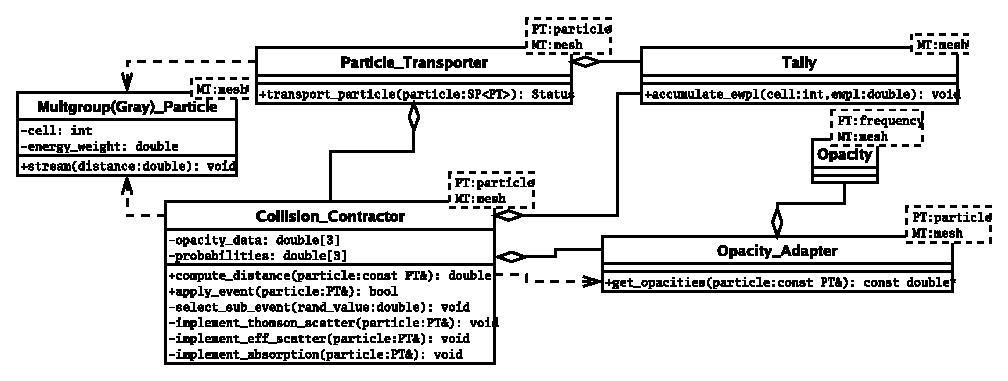
\includegraphics[width=6.5in]{figures/collision_contractor}
    \caption{Collision contractor implementation. Not all members shown} 
    \label{fig:collision_contractor}
  \end{figure}
\end{center}

Internally, it will use the opacity object to compute the distance and
the relative probabilities for its various sub-events.  If it wins,
the {\tt apply\_event} member function will dispatch to vartious
private members depending on the sub-event.

The contractor class can also aggregate the appropaite tally object
for the kinds of events that it handles as shown in the figure. This
removes more code from the transport algorithm itself.

The changes in particle state which occur with the collision events
depend on the state of the particle: Implicit versus Explicit
absorption. This is another source of complexity which can be moved
out of the transport algorithm. It is also another source of coupling
between the particle class and the contractor. If the model of
particle bahavior changes, then both the particle and the contractors
which depend on this model mush change. This problem also affects the
surface-tracking operations which need two methods for tallying
surface crossings depending on the absorption state of the particle. 

\subsection{Opacity Adapter}

One of the problems to address is the differing interface between the
{\tt Opacity} class for gray and multigroup frequency.  The multigroup
version contains an extra argument for the energy group of the
particle. We propose to wrap the opacity class with an adapter which
takes the particle as an argument and returns the correct opacity
information. This is also depicted in
Figure~\ref{fig:collision_contractor}. 

The {\tt Opacity\_Adapter} class will be specialized on the frequency
type (which is part of the type of the particle class). The
specialized versions will differ by containing the correct type of
opacity object, and extracting different data from the particle object
(cell and group versus just cell). They will fetch information from
the opacity object via the appropiate interface for the frequency
type.

The adapter class is used in by the collision event contractor, which
will also need to be templated on the frequency type of the particle.
This, in turn, implys that the particle transporter class itself needs
to be templated on this parameter.

In various classes we can choose between templating on the particle
type itself or just the frequency type. In making the transition
between the two, we need to be able to extract the frequency type from
the particle type, or build the particle type from the frequecny type
(by combining it with other type information, e.g. mesh type). We give
one likely assignment of template parameters in
Figure~\ref{fig:collision_contractor}. In this implementation, class
{\tt Opacity\_Adapter} extracts the frequency type partameter {\tt
  FT} from the particle type {\tt PT} to determine the correct
parameter for the {\tt Opacity} class. This can be facilitated by a
{\tt typedef} in the derived particle classes.

\subsection{A good design spoiled: The trouble with random walk}

The implementation of random walk introduces considerable complexity
into the particle transport algorithm. For example, random walk:

\begin{itemize}
\item Requires more data: 
  \begin{itemize}
  \item Depends on both the {\em distance} to census and the {\em
      time} to census.
  \item Uses more opacity information.
  \end{itemize}
  
\item Has more conditions on its execution:
  \begin{itemize}
  \item May be disabled
  \item Cell must be diffusive, e.g. the random walk radius dictated
    by the size of the cell must be greater than the number of mean
    free paths. 
  \item Random walk radius must lie between the computed distance to
    collision and the distance to census: $d_{\mbox{collision}} <
    r_{\mbox{\tiny RW}} < d_{\mbox{census}}$. 
  \item There must be no tally surfaces in the cell.
  \item Particle must have come from volume source or have just
    undergone effective scattering.
  \end{itemize}

\item  Does more to the particle:
  \begin{itemize}
  \item Kills particles that reach weight cutoff, 
  \item Sends particles still in radius straight to census.
  \item Changes position and direction of particle in a different
    manner than streaming.
  \end{itemize}
  
\item Interacts with frequency type: Change in particle weight is
  different.
  
\end{itemize}

The current implementation of random walk functionality,
e.g. determination of the random walk radius and application of the
random walk step is currently split between the {\tt Random\_Walk}
class, the {\tt Particle} base class and the two derived particle
classes. Our objective is to re-package the random walk functionality
in contractor form and take the responsibilities away from the
particle classes.

To do this, we propose a contractor-style facade to the {\tt
  Random\_Walk} class. This class will implement the {\tt
  compute\_distance} and {\tt apply\_event} methods taking a particle as
an argument. We divide up the responsibilities for random walk as
follows:

\begin{itemize}
\item The {\tt Particle\_Transporter} class will manage the
  interaction between random walk radius and other contractors. 
  This consists of the comparison of the random walk radius to the
  collision and census distances and disabling random walk in
  cells with tally surfaces. 
\item The {\tt Random\_Walk\_Contractor} class will implement members
  required in the contractor interface and all operations which apply
  directly to a particle . Frequency dependent parts of the
  implementation will be moved from the particle classes to the
  contractor.
\item Otherwise, functionality will remain in the existing {\tt
    Random\_Walk} class as much as possible, being modified to work
  with {\tt Random\_Walk\_Contractor} as necessary.
\end{itemize}

In the current implementation, the particle transport method
dispatches to two different implementations based on the existence of
a random walk object. This means that the check is performed only once
per particle to be transported. To unify these two different transport
implemetations, we must move this check to inside the main transport
loop, which means that it will be performed once per streaming step.
This is a small, but perhaps not unimportant performance penalty.

One way around this will be to statically bind the activation of
random walk using a template parameter. The feasiability of this will
be examinded further once the performance penalty is assesed.

\subsubsection{``Random-Walkability''}

Random walk can only be executed if the particle is volume source or
has just undergone effective scattering. These states are part of the
enumeration of states in the current particle class.  Effective
scattering is a subset of the collision event. Rather than frame the
conditional on random walk in terms of all possible states which make
random walk permissible, we seek to create a single particle state
which is synonymous with ``random-walkability''. Additional
contractors will have the responsibility to set or not set this state
of the particle as appropriate.

This means that part of the interaction between contractors is being
handled outside of the main particle transport loop. The alternative
is to make ``random-walkability'' a property tracked in the main
loop. This adds to to communication required with contractors, e.g. (to
determine if the collision event satisifies
``random-walkability''). At the risk of obscuring the interaction
between contractors, we prefer an implemention using particle state
modified by contractors in a first pass to this problem. 

``Random-walkability'' appears to be equivalent to the particle's
current direction being sampled from an isotropic distribution. In the
current multigroup particle implementation effective scattering events
result in sampling an isotropic distrubution for the direction. The
Grey particle implemetation seems to be fudging on this a bit. It does
not have an effective scatter method and uses the base particle
scatter method instead. This also appears to be an isotropic scatter,
but is implemented differently.

If indeed ``Random-walkability'' == ``current direction was sampled
isotropically'' then we can use the code which samples the new
direction for the particle to set the particle state as well. It will
also be necessary for all other contractors which cause the direction
to be sampled in a non-isotropic fasion to set the state variable to
false. We revisit the implementation of state variables in
Section~\ref{sec:State}. 

\subsubsection{Executing Random Walk}

Random walk sends particles directly to census if they remain within
the radius. If a particle exits the random walk sphere, but it's new
weight is below cutoff, it is killed instead of switching to analog
absorption mode. 

There are two ways of implementing the effects of random walk:
\begin{enumerate}
\item Dispatch to these actions in the particle transport function.
  The random walk contractor would set a flag (possibly inside the
  particle) indicating it's post-random walk fate.
  
\item Have the random walk implementation perform the actions on the
  particle itself. The means that the random walk contractor needs to
  know how to send a particle to census or to kill it. If there are
  free functions or contractors which perform these actions, then the
  random walk contractor can invoke them directly.
\end{enumerate}

Method 1 requires fewer interactions between contractors, but results
in a more complicated particle-transport function. Method 2 is
considered to be more in the spirit of the contractor model. In this
implemetation, the main particle transport responsibilities are
limited to contractor solicitation and interaction. 

\subsection{Extrinsic Surface Tracking} \label{sec:surface_tracking}

The process of tracking particles which cross extrinsic surfaces
(e.g. surfaces overlaid onto the mesh) is another source of
complication in the particle transport algoirhtm. The implementation
of crossing detection is a post-processing step after a particle
streams. Thus, it disables random walk in cells where a tally surface
is present. Moreover, after a random walk, there is no need to check
for surface crossings.

Surface tracking also introduces more instances of code duplication.
The exponential decay of the weight of a particle undergoing implicit
absorption is implemented in both the particles streaming operation,
and in the surface tracking classes to determine the weight at the
crossing point. Also, the surface tracking class must behave
differently depending on the streaming mode of the
particle. Furthermore, the final position of the particle is computed
both in the stream operation and in the surface tracking.

To eliminate this duplication, we need to pull the weight and final
position computations out of the particle class and put it in a place
available to both update the weight and final position of the particle
and for use in the surface tracking. 

\subsection{Whither Particle?}

The particle classes have been stripped of much of their functionality
at this point, since they no longer perform the transport
operations. Their remaining responsibilities are limited to the
following:
\begin{itemize}
  \item Have a position and direction of travel. 
  \item Know which cell of the mesh the position is in.
  \item Know the energy weight and absorption mode.
  \item Know the remaining travel distance to the end of the
    time-step.
  \item (MG only) know which energy group the particle is in.
  \item Have a random number state and provide random numbers to
    contractors.
  \item Be able to pack all of the information in the particle state
    into a {\tt vector<char>} for communication.
  \item Know how to stream a given distance by modifying the position
    and adjusting the energy weight according to the absorption state.
\end{itemize}

The particle is beginning to look more like a plain data-holder. In
light of the code duplication discussed in
Section~\ref{sec:surface_tracking}, we may want to remove the
streaming functionality from particle and bestow it upon a streaming
operator. This streaming operator would modify the state of the
particle according to the abosprtion state and provide the necessary
information to the extrinsic surface tracker.

The ever-expanding enum in the particle class should also be either
eliminated entirely or stripped down to contain just a few essential
states that need to be communicated between contractors.

\subsection{Matters of particle state} \label{sec:State}

There are several problems with the all-encompasing enumerated state
of the current particle class. It is {\em excessivly specific}
including states which should be just internal details of various
event implementations. It {\em breaks encapsulation} by exposing
intertnal details that external code should not know about. Worst of
all it is {\em brittle}, since changes in the state enumeration
require updating the tedius string conversion routines and examining
all other pieces of code which might conciveably depend on the exact
state of the particle.

We seek to replace the enumerated state of the particle with a more
svelte version. States which are internal details of events will be
handled by the event contractors. All that we're left with are states
which coordainte the interactions between contractors or which are
otherwise effected by or affect the behavior of more than one
contractor.

\subsubsection{Creeping state scope}

One problem with using particle state to handle interaction between
contractors is that the manipulation of a given state tends to spread
from the contractors directly involved to all of the others.  Our
working example for this problem is random walk. We expect the same
kind of issues with DDIMC.

The central issue is that we cannot constrain {\em a priori} the
number of contractors which may effect or be affected by a given
detail of the particle state. For random walk, this means that all
contractors which re-sample the direction of the particle must know
about the ``random-walkability'' particle state variable and modify it
appropiately.

The solution to this problem, as with all others in computer science,
is to add another layer of indirection. The contractors themselves can
dispatch to a layer which performs the actual implementations, e.g. of
direction sampling. By encapsulating the actions which affect the
particle, we can guarantee that the other particle state variables are
kept in sync.

For DDIMC, (discussed further in Section~\ref{sec:DDIMC}), the
particle state which is likely to matter is whether the particle has
just crossed a mesh boundary. This is a state that will automatically
expire (``become false'') if any {\em other} kind of action is
performed on the particle. This suggests that some aspects of the
particle state should automatically expire and only explicitly be set
to ``true''.  The expiration of state would need to occur after it has
had a chance to be useful, i.e. after the bid solicitation stage in
the coordinator. This means that the right point to clear the state of
the particle is between the bid solicitation and implementation
stages.

\subsubsection{Mutually exclusive or orthogonal?}

The current and anticiapted future implementation requires two
additional pieces of state information which correspond to
``random-walkability'' and ``DDIMC-ability''. Physcially, these appear
to correspsond to ``direction sampled isotropically'' and ``just
entered a new cell''. These physical states appear to be mutually
exclusive, since the operation of moving a particle across a mesh
boundary will not cause it's direction to be resampled, and vice
versa. Does this mean that we should make the particle states mutally
exclusive as well?

In the design, this would suggest an enumeration of the possible
states of the particle, restricting the particle only one at a time.
This enumeration would also contain a ``none'' state, which would be
attained after a state reset. The orthogonal decomposition of states
would use independent boolean variables to indicate the truth of each
one.

We prefer the orthogonal decomposition of states with boolean
variables for one primary reason: Additional states added for other,
currently unforseen, events may break the independence the exclusive
model relies on.

\subsubsection{Inside or outside the particle?}

We also consider moving these supplemental state variables for
contractor interactions outside the particle and into a seperate
class. This class would be passed along with the particle to the
distance calculation and a new state object would be returned by the
contractors.

This gives the particle one less reason to change by isolating it from
the contractors that are working on it. It even makes it easier to use
the particle class with a wholly different set of contractors, or with
none, in other applications. Only the supplemental state-holding class
would need to be modified.  This also eliminates the awkward ``forget
old state'' operation in the coordinator by replacing the old state
with a fresh one generated by the winning contractor.

With the ``interaction state variables'' move outside, the particle
would also contain just exactly the information that it needs to carry
with it between problem domains, bringing it more in line with it's
new life as a data container. For example, the ``Analog versus
Implicit'' absorption state belongs firmly within the particle class
since it needs to be communicated along with it, and while it affects
the behavior of some contractors, it isn't really about interaction
between contractors.

With a seperate state object, the contractor interface would look as
follows:

\begin{verbatim}
  double compute_distance(const PT& particle, const State& state)
  State apply_event(PT& particle)
\end{verbatim}

The State class could be defined outside the Particle transport class
and so available too all of the contractors. It could also be a formal
template parameter of the contractors.  The state object would be
local to the particle transport function. 

We use a return value of the state in {\tt apply\_event} since we
suppose that this will not be an expensive object to copy. This
accomplishmes the erasure of the old state and assignment of the new
one in one step. The state object also replaces the ambigously
necessary ``bool'' as the return type of {\tt apply\_event}.

These are all nice and compelling reasons for a separate state object,
but another class may be overkill here.

\section{Doing particle transport with contractors}
\label{sec:particle_transport}

\subsection{The particle transport algorithm}

\begin{figure}[htb]
  \fbox{
    \parbox[b]{6.4in}{
      \begin{itemize}
      \item Accept a new particle for transporting
      \item Initialize the extrinsic surface tracker
      \item While the particle is active:
        \begin{itemize}
        \item Get distance to collision $d_{\mbox{collide}}$.
        \item Get distance to census $d_{\mbox{census}}$.
        \item If Random walk is feasible, i.e:
          \begin{itemize}
          \item Random walk is enabled,
          \item No tally surface in cell,
          \item Particle is ``random-walkable'', 
          \end{itemize}
          Then...
          \begin{itemize}
          \item Get random walk distance $r_{\mbox{\tiny RW}}$ from
            the mesh.
          \item Compute the mean free paths (mfp) from the opacity.
          \item If $d_{\mbox{collide}} < r_{\mbox{\tiny RW}} <
            d_{\mbox{census}}$, and $r_{\mbox{\tiny RW}} >
            \mbox{mfp}$, call the random walk implementor.
          \end{itemize}
        \item If we {\bf did not} do random walk, we must be streaming, so:
          \begin{itemize}
          \item Get distance to mesh crossing $d_{\mbox{mesh}}$.
          \item Get distance to weight transition $d_{\mbox{weight}}$.
          \item Determine the smallest element of $d_{\mbox{collide}},
            d_{\mbox{census}}, d_{\mbox{mesh}}, d_{\mbox{weight}}$.
          \item Dispatch the particle to the owner of the winning
            distance.
          \item Do surface tracking check.
          \end{itemize}
        \end{itemize}
      \item Return the particle and it's status to the caller
      \end{itemize}
    }
  }
  \caption{The particle transport algorithm}
  \label{fig:particle_transport}
\end{figure}

Figure~\ref{fig:particle_transport} contains the main-loop of the
particle transport algorithm using contractors. The various
implementation actions are not shown, since these are handeled by the
contractors. One difference between the top level organization in this
version and the existing transport algorithm is that we have moved the
execution of random walk up into the same conditional as the selection
of random walk. This reduces the number of conditionals on random
walk. We exit the conditional with a break and return to the top of
the while loop. This is done in order to avoid putting the rest of the
streaming steps inside of a conditional.

The {\tt transport\_particle} member of the particle transporter class
returns an object of class {\tt Status}. The purpose of this object is
to convey enough inforation so that the caller can decide what to do
next with the particle. In applications, the caller will be the
asynchronous transport implementation which currently calls the
particle transport function. Once the particle-transport stage is
completed, a particle might need to be added to the census,
communicated to another processor, or be dead. We need to return
enough information from the particle-transport algortihm to determine
what to do next. It is possible that a simple boolean will suffice.

\subsection{Persistence and aggregation of objects}

There are more objects involved when using the contractor metaphor for
particle transport, which introduces some new issues. The lifetime of
the contractors must be managed, as well as the other objects they
collaborate with. Also, the means by which objects are aggregated must
be determined.

As a first solution to the problem, we propose building all of these
objects at a level above particle transport, e.g. at the asynchrous
transport algorithm level. Smart pointers can be used to manage the
lifetime of these objects. Since the relationship between the {\tt
  Particle\_Transporter} and it's contractors will not change during
the lifetime of these objects, they can be connected by holding
references to the contractors established at construction. Likewise
the contractors can be constructed with references to the objects that
they need to collaborate with. Consequently, most of the aggregation
relationips in the between objects will be implemented through
references instead of pointers. This will keep down the pointer
de-referenceing overhead.

\section{Proposed sequence for refactoring}

Our first objective for this sub-project is to unify the four
implementations of the particle transport algorithm. On outline of our
proposed approach to do so are as follows.

\begin{enumerate}
\item Unify the logic between the random-walk and non-random walk
  transport versions. 

  \begin{itemize} 
  \item Group the detection and execution of random walk
    together. 
  \item Wrap the random walk detection/execution in a conditional
    (This can be done via conditionals on the {\tt Random\_Walk} smart
    pointer.
  \item At this point, it should be possible to combine the two
    functions.
  \end{itemize}
  
\item Create {\tt Particle\_Transporter} class. This class will take
  over the particle transport operation.

  \begin{itemize}
  \item Template the class on the frequency type (FT) or the full type
    of the particle (PT).
  \item Copy over specialized versions of the transport algorithm in
    the particle-transporter for the different frequency types from
    the particle classes.
  \item Expand the public interface of the Particle classes as
    necessary, to enable the transport methods in the
    particle-transporter to function. Various other methods of the
    Particle class can also be moved over to the transporter as
    needed.
  \item Construct the particle-transporter with references or pointers
    to classes which provide needed information, e.g. opacity, mesh.
  \end{itemize}

  Once {\tt Particle\_Transporter} is in place, modify the Particle
  unit tests to use it instead of the particle's transport method.
  
\item Unify the Gray and Multigroup specializations in the particle
  transporter by creating a collision event contractor class: {\tt
    Collision\_Contractor}

  \begin{itemize}
    \item Create class and template on particle type
    \item Implement {\tt compute\_distance} and {\tt apply\_event}
    \item Construct with and aggregate required assistant classes.
      e.g.  {\tt Opacity\_Interface}.
    \item Modify {\tt Particle\_Transporter} to use {\tt
        Collision\_Contractor}.
    \item The Gray and Multigroup specializations of the transport
      function should now differ only in symbolic types, so we can
      eliminate the specializations.
    \end{itemize}
    
  \item Create a contractor for Random Walk. 

    \begin{itemize}
    \item Wrap the current {\tt random\_walk} class in a
      contractor-style adapter which specilizes on frequency
      type. This contractor will also implement a method to determine
      if random walk is possible.
    \item Move the distance computation and implemetation methods up
      from the random walk object or down from the particle class into
      this contractor.
    \item Move the interaction logic between random walk and other
      limiting events into the particle transport loop or the
      contractor's ``is random walk possible'' method, as appropiate.
    \end{itemize}

    Modify {\tt Particle\_Transporter} to use this contractor.
    
  \item Create a contractor for mesh crossing events.
    
    This should be easy after the last two. Modify {\tt
      Particle\_Transporter}.

  \item Evaluate the use of a contractor to handle going to census and
    weight cutoff. These may be simple enough to implement as free
    functions or as part of {\tt Particle\_Transporter}.
    
  \item Remove the old transport methods in particle classes. Remove
    unnecessary data types and data objects.
    
  \item Modify clients of particle transport to create and use a {\tt
      Particle\_Transporter} instead of calling the particle's
    transport method.

\end{enumerate}

\section{Next Steps}

\subsection{Anticipating new features}

One of the motivations of this refactoring project is the anticipation
of several new features, which would be impossible to implement with
the particle transport algorithm in it's current state. We would like
to reassure ourselves that the new design is more amenable to the
addition of these features. 

\subsubsection{DDIMC} \label{sec:DDIMC}

DDIMC, another diffusion-based method, is likely to be added to the
particle transport algorithm soon. Like random walk, DDIMC replaces
the streaming steps of particle transport with a diffusion process in
suitable cells. Unlike random walk, it begins a soon as a particle
enters a sufficiently diffusive cell and propagates the particle until
it exits the cell.

We should allow for the possibility that DDIMC and random walk will be
active at the same time, so they will compete with each other for
control of the particle. Since DDIMC will propagate a particle all the
way through a cell, it should be attempted first. The physical
conditions on which it can be used are also like to be more stringent
than random walk, e.g. requiring the entire cell to be optically
thick.

The DDIMC operation transportes the particle to a boundary of the mesh
cell or sends it directly to census if it fails to escape in time.
Like random walk, which can shuffle particles directly to census or
premature death, DDIMC can directly pass particles to the mesh
crossing of census contractors after it is finished with them.

With the DDIMC option in place, the particle transport algorithm is
modified with another conditional layer. The result is presented in
Figure~\ref{fig:modified_particle_transport}. In this algorithm,
``DDIMC-able'' is the analog of ``Random-walkable'' and is probably
equivalent to having just performed a cell crossing. This is a
particle state variable which can be set by the mesh crossing
contractor. We also note that the net effect of adding DDIMC is to
push random walk and streaming down another level in the conditional
hierarchy.

\begin{figure}[htb]
  \fbox{
    \parbox[b]{6.4in}{
      \begin{itemize}
      \item Accept a new particle for transporting
      \item Initialize the extrinsic surface tracker
      \item While the particle is active:
        \begin{itemize}
        \item If DDIMC is feasible, i.e.:
          \begin{itemize}
          \item DDIMC is enabled.
          \item No tally surface in cell.
          \item Particle is ``DDIMC-able'',
          \item Cell is sufficiently opaque.
          \end{itemize}
          Then, call the DDIMC contractor implementation.
        \item If we {\bf did not} do DDIMC, we must be moving within the
          cell, so:
          \begin{itemize}
          \item Get distance to collision $d_{\mbox{collide}}$.
          \item Get distance to census $d_{\mbox{census}}$.
          \item If Random walk is feasible, i.e:
            \begin{itemize}
            \item As before...
            \end{itemize}
            Then...
            \begin{itemize}
            \item As before...
            \end{itemize}
          \item If we {\bf did not} do random walk, we must be streaming, so:
            \begin{itemize}
            \item Get distance to mesh crossing $d_{\mbox{mesh}}$.
            \item Get distance to weight transition $d_{\mbox{weight}}$.
            \item Determine the smallest element of $d_{\mbox{collide}},
              d_{\mbox{census}}, d_{\mbox{mesh}}, d_{\mbox{weight}}$.
            \item Dispatch the particle to the owner of the winning
              distance.
            \item Do surface tracking check.
            \end{itemize}
          \end{itemize}
        \end{itemize}
      \item Return the particle and it's status to the caller
      \end{itemize}
    }
  }
  \caption{The particle transport algorithm with DDIMC}
  \label{fig:modified_particle_transport}
\end{figure}

\subsubsection{Compton Scattering}

With the contractor framework in place, the addition of Compton
Scatting should be encapsulated with the collision contractor class
and transparent to the rest of the particle transport algorithm. One
way that this might fail is through additional interactions between
Compton Scattering and other contractors (a la, effective scattering
and random walk). This will have to be handeled through the addition
of appropiate state variables. 

\subsubsection{Material Motion}

No friggin' idea.

\subsection{More refactorings}

Some other changes to the code may follow logically after the
refactoring above is completed, or may be inserted as part of the
process. We list some of those here.

\begin{itemize}
\item Eliminate mesh dependency from Particle.

  Since the particle will no longer logically depend on the mesh, the
  mesh type template parameter can probably be removed from the
  particle type. Eliminating this dependency may make it possible to
  remove mesh depenence from other classes as well.
      
\item Collapse particle hierarchy. 
  
  Since most of the differing code will have been removed, the
  particle hierarchy is ripe for being collapsed into a single class.
  The new particle class would be templated on the frequency type and
  use a ``mixin'' style component to add the extra members needed by
  the multigroup type.

\item Statically bind random-walk
  
  We can look for a way to use template parameters to statically build
  versions of the particle-transport algorithm with and without random
  walk. Since these particle transporters will have different types,
  the algorithm would be called via and interface in an abstract base
  class. Since the virtual function call would only be at the
  beginning of the particle transport algorithm, the cost is likely
  negligible.
  
\item Statically bind surface-tracking. 

  As with random walk, we can use template parameter object to build
  two versions of the particle transport algorithm with and without
  surface tracking. Since surface tracking interacts with random walk,
  statically binding both may be impractically complicated. 

\item Clean up the random sampling methods.

  There appear to be different means of performing isotropic random
  samplings. These should be combined.

\end{itemize}

\subsection{Modifications inspired by the refactoring}

Some other, possibly beneficial, changes have come to light during the
analysis of this refactoring. Since they will change the bahavior of
the code, they must not be implemented concurrently with the refactoring.

\begin{itemize}

\item Eliminate cutoff as a limiting event.

  Weight-based cutoff can be changed from a limiting event to a stream
  post-processing event. This will speed up transport, since the
  distance to cutoff computation is logarithmic. It will also simplify
  the particle-transport loop somewhat.

\item Modify random walk. 
  
  More random walk steps can be taken if the radius is limited by the
  distance to census, instead of skipping it when the radius exceedes
  the census distance. 

  Also, the random walk raidus could be limited to the distance to a
  tally surface, instead of completely disabling random walk in cells
  which contain a tally surface. 

  The cell size, distance to census and distance to tracking surface
  could all be combined into geometric limiters on the random walk
  radius (indeed, the distance to cell boundary and distance to
  tracking surface are conceptually very similar). The random walk
  radius would be chosen as the minimum of these geometric
  contstraints and random walk would be implemented if this radius is
  larger than the distance to collision and mean free path quantity.

\end{itemize}
  
\newpage
\bibliography{jayenne_ref}
\bibliographystyle{plain}
 
\closing
\end{document}

%%---------------------------------------------------------------------------%%
%% end of refactor_planning.tex
%%---------------------------------------------------------------------------%%
